%%%%%%%%%%%%%
% LECTURE 4 %
%%%%%%%%%%%%%
\vspace{1cm}

\noindent \lecture{4}{15/10/2021}

\vspace{0.5cm}

\noindent Continuiamo la discussione riguardante il concetto di entanglement. Dato che questo fenomeno si manifesta in sistemi con almeno due qubit, possiamo utilizzare due differenti basi:
\begin{itemize}
    \item \textbf{Base computazionale} (o \textbf{standard}): formata dagli stati $\lbrace \ket{00}, \ket{01}, \ket{10}, \ket{11} \rbrace$ (la due entrate indicano gli stati del primo e secondo qubit rispettivamente).
    
    \item \textbf{Base di Bell} (o \textbf{EPR}): costituita dagli stati 
    \begin{align*}
        \ket{\beta_{00}} &= \frac{1}{\sqrt{2}} (\ket{00} + \ket{11}) \, , &\ket{\beta_{01}} &= \frac{1}{\sqrt{2}} (\ket{01} + \ket{10}) \, , \\
        \ket{\beta_{10}} &= \frac{1}{\sqrt{2}} (\ket{00} - \ket{11}) \, , &\ket{\beta_{11}} &= \frac{1}{\sqrt{2}} (\ket{01} - \ket{10}) \, ;
    \end{align*}
    notiamo che si trattano di stati entangled costruiti a partire da combinazioni lineari indipendenti degli stati della base computazionale.
\end{itemize}

\noindent Chiaramente, trattandosi di una base, possiamo espandere qualsiasi stato $\ket{\psi}$ nella base EPR, scrivendo
\begin{equation*}
    \ket{\psi} = \sum_{n,m=0}^1 \alpha_{nm} \ket{\beta_{nm}} \, .
\end{equation*}
Conseguentemente, se si cerca la probabilità di trovarsi in $\ket{\beta_{nm}}$ si può effettuare una misurazione nella base di Bell e ottenere $P(\ket{\beta_{nm}}) = \abs{\alpha_{nm}}^2$. 

\noindent Gli stati della base di Bell non sono difficili da costruire utilizzando i gate che abbiamo visto precedentemente. Supponiamo di poter utilizzare un computer quantistico i cui qubit si trovano nella base standard $\lbrace \ket{0}, \ket{1} \rbrace$. Utilizziamo l'\texttt{H-gate} e il \texttt{CNOT-gate}: 
\begin{itemize}
    \item Ricordiamo che $H\ket{0} = \ket{+}$ e $H \ket{1} = \ket{-}$, quindi il gate di Hadamard permette di passare da un qubit nella base computazionale ad un qubit in una combinazione lineare di elementi di questa base (si ricordi la matrice in \eqref{Hadamard_matrix} e le definizioni in \eqref{basi_di_sigma_12}). 
    
    \item Il \texttt{CNOT-gate}, invece, scambia il secondo qubit solamente se il primo si trova in $\ket{1}$:
    \begin{align*}
    \ket{00} &\overset{\texttt{CNOT}}{\longrightarrow} \ket{00} \, , &\ket{01} &\overset{\texttt{CNOT}}{\longrightarrow} \ket{01} \, , \\
    \ket{10} &\overset{\texttt{CNOT}}{\longrightarrow} \ket{11} \, , &\ket{11} &\overset{\texttt{CNOT}}{\longrightarrow} \ket{10} \, .
\end{align*}
\end{itemize}

\noindent Utilizzando questi due gate possiamo facilmente implementare il circuito seguente 
\begin{center}
    \mbox{
        \Qcircuit @C=2em @R=1.5em {
            \lstick{\ket{x}} & \gate{H} & \ctrl{1} & \qw \\
            \lstick{\ket{y}} & \qw & \targ & \qw
        }
    }
\end{center}
i cui output sono esattamente gli stati $\ket{\beta_{xy}}$ della base di Bell. Verifichiamolo:
\begin{align*}
    \ket{00} &\overset{H}{\rightarrow} \frac{1}{\sqrt{2}} (\ket{0} + \ket{1}) \otimes \ket{0} = \frac{1}{\sqrt{2}} \left( \ket{00} + \ket{10} \right) \overset{\texttt{CNOT}}{\rightarrow} \frac{1}{\sqrt{2}} \left( \ket{00} + \ket{11} \right) \equiv \ket{\beta_{00}} \, , \\
    \ket{01} &\overset{H}{\rightarrow} \frac{1}{\sqrt{2}} (\ket{0} + \ket{1}) \otimes \ket{1} = \frac{1}{\sqrt{2}} \left( \ket{01} + \ket{11} \right) \overset{\texttt{CNOT}}{\rightarrow} \frac{1}{\sqrt{2}} \left( \ket{01} + \ket{10} \right) \equiv \ket{\beta_{01}} \, , \\
    \ket{10} &\overset{H}{\rightarrow} \frac{1}{\sqrt{2}} (\ket{0} - \ket{1}) \otimes \ket{0} = \frac{1}{\sqrt{2}} \left( \ket{00} - \ket{10} \right) \overset{\texttt{CNOT}}{\rightarrow} \frac{1}{\sqrt{2}} \left( \ket{00} - \ket{11} \right) \equiv \ket{\beta_{10}} \, , \\
    \ket{11} &\overset{H}{\rightarrow} \frac{1}{\sqrt{2}} (\ket{0} - \ket{1}) \otimes \ket{1} = \frac{1}{\sqrt{2}} \left( \ket{01} - \ket{11} \right) \overset{\texttt{CNOT}}{\rightarrow} \frac{1}{\sqrt{2}} \left( \ket{01} - \ket{10} \right) \equiv \ket{\beta_{11}} \, ;
\end{align*}
si noti come l'azione di un gate (in questo caso l'\texttt{H-gate}) su un singolo qubit non basti per produrre uno stato entangled. Al contrario il \texttt{CNOT-gate}, invece, crea stati entangled poiché agisce su coppie di qubit. 

\noindent Vediamo ora due esplicite applicazioni dell'entanglement. 

\section{Superdense coding}
Si tratta del primo esempio esplicito delle potenzialità dei metodi quantistici contro i metodi classici. Il problema riguarda il come inviare informazioni di due bit classici (00, 01, 10, 11) ad un generico sperimentatore. Consideriamo la sperimentatrice Alice e supponiamo che abbia due bit di informazione (due numeri $xy$) e che voglia inviarli allo sperimentatore Bob. Dal punto di vista classico, Alice semplicemente utilizza un canale classico (un telefono ad esempio) per comunicare direttamente a Bob quale coppia di numeri possiede. Nel caso in cui Alice possieda due qubit, invece, può inviare solamente uno dei due sfruttando il fatto che siano entangled. Supponiamo che Alice e Bob condividano due qubit entangled, ad esempio
\begin{equation*}
    \ket{\psi} = \frac{1}{\sqrt{2}} \left( \ket{00} + \ket{11} \right) = \ket{\beta_{00}} \, ,
\end{equation*}
dove Alice possiede il primo qubit (prima entrata del ket) e Bob il secondo. Cosa deve fare Alice per inviare solamente un singolo "pezzo" di informazione? Ad esempio Alice può effettuare una qualche operazione sul suo qubit e, sfruttando l'entanglement, Bob sarà in grado di leggere l'informazione desiderata (la coppia di numeri $xy$ che Alice vuole inviare) facendo una singola misurazione. Più precisamente, supponiamo che Alice voglia inviare delle informazioni effettuando le seguenti operazioni sul proprio qubit di $\ket{\psi}$:
\begin{equation*}
    \text{Alice invia:} \; 
    \begin{cases}
        00 \, , &\text{non fa niente} \\
        10 \, , &\text{applica } Z \\
        01 \, , &\text{applica } X \\
        11 \, , &\text{applica } ZX
    \end{cases} \, .
\end{equation*}
Cosa succede allo stato condiviso quando applica queste operazioni? 
\begin{itemize}
    \item Quando vuole inviare 00 non effettua alcuna operazione quindi $\ket{\psi} \rightarrow \ket{\psi} = \ket{\beta_{00}}$. 
    
    \item Nel caso in cui decide di inviare 10 applica $Z$:
    \begin{equation*}
        \ket{\psi} \rightarrow Z \frac{1}{\sqrt{2}} \left( \ket{00} + \ket{11} \right) = \frac{1}{\sqrt{2}} \left( \ket{00} - \ket{11} \right) = \ket{\beta_{10}} \, .
    \end{equation*}
    
    \item Quando invece vuole inviare 01 applica $X$:
    \begin{equation*}
        \ket{\psi} \rightarrow X \frac{1}{\sqrt{2}} \left( \ket{00} + \ket{11} \right) = \frac{1}{\sqrt{2}} \left( \ket{10} + \ket{01} \right) = \ket{\beta_{01}} \, .
    \end{equation*}
    
    \item Infine se vuole inviare 11 applica $ZX$:
    \begin{equation*}
        \ket{\psi} \rightarrow ZX \frac{1}{\sqrt{2}} \left( \ket{00} + \ket{11} \right) = Z \frac{1}{\sqrt{2}} \left( \ket{10} + \ket{01} \right) = \frac{1}{\sqrt{2}} \left( \ket{01} - \ket{10} \right) = \ket{\beta_{11}} \, .
    \end{equation*}
\end{itemize}

\noindent Effettuando queste operazioni, Alice è in grado di spedire ciò che vuole: $xy \rightarrow \ket{\beta_{xy}}$. Bob può effettuare una (singola) misura nella base di Bell, stabilire quale dei 4 stati possiede, %Qui risiede l'idea di \textbf{non-località} della QM: sebbene Bob possa trovarsi molto lontano da Alice, il suo qubit è cambiato a seguito delle operazioni di lei e può 
e leggere quindi i bit corrispondenti $xy$. L'informazione classica corrispondente a due bit \`e stata inviata attraverso un solo qubit.

\noindent Questo esempio, nonostante sia un po' accademico, risulta particolarmente interessante perché mette in risalto come, grazie all'entanglement, sia possibile ridurre il numero di operazioni necessarie per inviare un'informazione rispetto al caso classico. 

\section{Teleportation}
Innanzitutto che cosa intendiamo con il termine \textit{teletrasporto}? In questo contesto viene inteso con il significato di ricostruire un qubit molto lontano da dove si trovava in origine: il qubit originale sparisce e una sua nuova copia viene creata altrove. L'idea è quella di effettuare questa particolare ricostruzione usando solamente operazioni classiche sui qubit.

\noindent Supponiamo che Alice (d'ora in avanti chiameremo sempre in questo modo i nostri due sperimentatori) abbia un generico qubit $\ket{\psi} = \alpha \ket{0} + \beta \ket{1}$ e che voglia inviarlo a Bob senza utilizzare alcun canale quantistico. Dalle leggi della QM sappiamo che non possiamo estrarre sia $\alpha$ che $\beta$ con una singola misura e inoltre non è possibile clonare questo stato generico. Inoltre, se volesse inviare direttamente questo stato con assoluta precisione (assumiamo $\alpha , \beta \in \mathbb{R}$) mediante un canale classico, allora necessiterebbe due stringhe infinite di bit e quindi del tempo infinito per inviarle. Come nel caso precedente, assumiamo che Alice e Bob condividano lo stato entangled $\ket{\beta_{00}} = \frac{1}{\sqrt{2}} \left( \ket{00} + \ket{11} \right)$, dove il primo qubit è di Alice e il secondo di Bob. Notiamo che Alice possiede due qubit: il qubit generico $\ket{\psi}$ che vuole teletrasportare e il qubit entangled con quello di Bob. Lo stato iniziale non è quindi altro che
\begin{equation}\label{teleportation_initial_state}
    \left( \alpha \ket{0} + \beta \ket{1} \right) \ket{\beta_{00}} = \frac{\alpha}{\sqrt{2}} \ket{0} \left( \ket{00} + \ket{11} \right) + \frac{\beta}{\sqrt{2}} \ket{1} \left( \ket{00} + \ket{11} \right) \, .
\end{equation}
Alice sottopone gli stati in suo possesso al seguente circuito:
\begin{center}
    \mbox{
        \Qcircuit @C=1em @R=1em {
            \lstick{\ket{\psi}} & \ctrl{1} & \gate{H} & \qw & \rstick{\text{Alice}} \\
            \lstick{} & \targ & \qw & \qw & \rstick{\text{Alice}} \\
            \lstick{} & \qw & \qw & \qw & \rstick{\text{Bob}}
            \inputgroupv{2}{3}{1.4em}{1em}{\ket{\beta_{00}}\; \; \; \;}{2em}
        }
    }
\end{center}
dove si è indicato in output a chi appartiene quel determinato qubit. Esplicitamente, si applica \texttt{CNOT-gate} ai due qubit di Alice in \eqref{teleportation_initial_state}:
\begin{equation*}
    \frac{\alpha}{\sqrt{2}} \ket{0} \left( \ket{00} + \ket{11} \right) + \frac{\beta}{\sqrt{2}} \ket{1} \left( \ket{10} + \ket{01} \right)  \, ;
\end{equation*}
dopodiché viene applicato \texttt{H-gate} al primo qubit di Alice:
\begin{equation*}
    \frac{\alpha}{2} (\ket{0} + \ket{1}) \left( \ket{00} + \ket{11} \right) + \frac{\beta}{2} (\ket{0} - \ket{1}) \left( \ket{10} + \ket{01} \right) \, ;
\end{equation*}
infine possiamo riscrivere l'espressione nel modo seguente
\begin{equation*}
    \frac{1}{2} \bigg[ \ket{00} (\alpha \ket{0} + \beta \ket{1}) + \ket{01} (\alpha \ket{1} + \beta \ket{0}) + \ket{10} (\alpha \ket{0} - \beta \ket{1}) + \ket{11} (\alpha \ket{1} - \beta \ket{0}) \bigg] \, ,
\end{equation*}
dove in questo ultimo passaggio abbiamo svolto i conti e riordinato l'espressione focalizzandoci su ciò che è posseduto da Alice (i due qubit di fronte alle 4 parentesi tonde) e da Bob (stato nella parentesi tonda). Consideriamo ora la Tabella \ref{tab:teleportation}: Alice può effettuare una misura nella base computazionale e dire a Bob (mediante un canale classico) ciò che ha ottenuto; dopo la misura lo stato collassa e Bob, a seconda del risultato, può effettuare o meno un'opportuna operazione sul proprio stato per ricostruire precisamente ciò che si voleva teletrasportare. 

\begin{table}[!ht]
	\centering
    \begin{tabular}{ccc}
        \toprule
        \text{Alice misura} & \text{Bob trova} & \text{Bob applica}  \\
        \midrule
        $\ket{00}$ & $\alpha \ket{0} + \beta \ket{1}$ & \text{Nulla} \\
        $\ket{01}$ & $\alpha \ket{1} + \beta \ket{0}$ & $X$ \\
        $\ket{10}$ & $\alpha \ket{0} - \beta \ket{1}$ & $Z$ \\
        $\ket{11}$ & $\alpha \ket{1} - \beta \ket{0}$ & $ZX$ \\        \bottomrule
    \end{tabular}\\
    \caption{Una volta che Alice effettua la propria misura nella base computazionale e dice a Bob ciò che ha ottenuto, quest'ultimo può applicare una precisa operazione per ricostruire lo stato $\ket{\psi}$ che Alice voleva teletrasportare. Si noti che, in tutti e quattro i casi, lo stato finale che ha Bob è sempre $\ket{\psi}$ indipendentemente dal risultato di Alice.}
    \label{tab:teleportation}
\end{table}

\noindent Un fatto fondamentale da evidenziare è che solamente informazioni classiche sono state trasferite tra Bob e Alice poiché tutto il resto (misurazioni e operazioni sugli stati) viene svolto localmente nel laboratorio: non c'è né violazione della relatività speciale in quanto non avviene alcun trasferimento di informazioni più veloce della luce, né violazione del teorema di no-cloning perché, una volta che Bob ottiene $\ket{\psi}$, Alice non possiede più lo stato che voleva teletrasportare. Si tratta solamente di un modo ingegnoso per sfruttare l'entanglement. 

\section{Disuguaglianze di Bell}
L'argomento delle disuguaglianze di Bell è un tema molto vasto che comprende moltissime disuguaglianze testabili sperimentalmente: ciò che accomuna tutte le misurazioni è la profonda differenza tra il concetto di probabilità \textit{classica} e \textit{quantistica}. Nella prima metà del '900, dopo la nascita della QM e i conseguenti trionfi che tale teoria era in grado di riportare, molti fisici, tra cui lo stesso Einstein, erano profondamente insoddisfatti del concetto intrinseco ed inevitabile di probabilità che permea tale teoria. In particolare, coloro che non accettavano la QM come teoria completa, credevano che il suo comportamento fosse in realtà dovuto alla nostra ignoranza su teorie ancora più fondamentali. Questo gruppo di persone credevano che le \textbf{osservabili}, in fisica, dovessero sempre soddisfare 2 requisiti base:
\begin{itemize}
    \item \textbf{Realismo}: un'osservabile deve avere un valore definito anche prima che la misura sia effettuata.
    
    \item \textbf{Località}: un esperimento effettuato in un ben preciso luogo ha solamente un effetto locale perché non può in alcun modo modificare risultati e comportamenti di altri esperimenti effettuati in regioni causalmente disconnesse. L'entanglement, ad esempio, è in profondo contrasto con il concetto di località. 
\end{itemize}

\noindent Nel corso di quegli anni furono svolti numerosi tentativi di riscrivere la QM in maniera tale che soddisfacesse i requisiti precedenti. Ad esempio, furono utilizzate le cosiddette \textbf{teorie delle variabili nascoste}. Tali teorie si basano sull'assunto secondo cui quando si misura un valore $a$ di un'osservabile $A$, in realtà il risultato della misurazione è incompleto perché l'intera teoria prevede l'esistenza di un'altra variabile $\lambda$ \textit{nascosta} ed inaccessibile. Se si potesse conoscere $\lambda$ allora si potrebbe predire qualsiasi cosa in maniera del tutto deterministica. Nonostante ciò, il concetto di probabilità in QM vìola queste regole e, come vedremo tra poco, utilizzando le disuguaglianze di Bell è possibile rilevare sperimentalmente tale violazione. 

\begin{esempio}[Singolo qubit]
    Consideriamo nuovamente il caso di un qubit e immaginiamo di trovarci nello stato $\ket{0}$. Nella Sezione \ref{sec:osservabili} abbiamo visto che il più generale operatore hermitiano che agisce su un singolo qubit è dato da una combinazione lineare di matrici di Pauli (non consideriamo l'identità), ossia $\vec{\sigma} \cdot \vec{n}$ dove $\abs{\vec{n}} = 1$. Supponiamo che a seguito di una misurazione possiamo ottenere $\vec{\sigma} \cdot \vec{n} \ket{\vec{n}} = \ket{\vec{n}}$ e $\vec{\sigma} \cdot \vec{n} \ket{-\vec{n}} = - \ket{-\vec{n}}$, quindi il risultato è $\pm 1$. Perciò, ricordando la decomposizione $\ket{0} = c_1 \ket{\vec{n}} + c_2 \ket{-\vec{n}}$, la probabilità di misurare 1 è $P(\vec{\sigma} \cdot \vec{n} = 1) = \abs{c_1}^2 = \abs{\braket{0}{\vec{n}}}^2$. Al tempo stesso sappiamo anche che il generico qubit si scrive come in \eqref{generic qubit}, quindi $\vec{n}$ può essere specificato scegliendo gli angoli $\theta$ e $\phi$: dato che avevamo sottolineato che $\vec{\sigma} \cdot \vec{n} \ket{\psi} = \ket{\psi}$ allora la soluzione che cerchiamo è $\ket{\vec{n}} = \ket{\psi}$, quindi
    \begin{equation*}
        P(\vec{\sigma} \cdot \vec{n} = 1) = \abs{\braket{0}{\vec{n}}}^2 = \abs{\braket{0}{\psi}}^2 = \cos^2 \! \left( \frac{\theta}{2} \right) \, .
    \end{equation*}
    Vediamo se riusciamo a riprodurre la medesima distribuzione di probabilità utilizzando una teoria classica basata sulle variabili nascoste. Supponiamo che, oltre allo spin, la particella sia in realtà descritta da un'extra variabile $\lambda$: tutte le particelle sono specificate dalla coppia fissata $(a = \pm 1, \lambda)$, ossia hanno spin $a = \pm 1$ e un preciso valore di $\lambda$ persino prima di effettuare la misurazione. Per semplicità assumiamo $\lambda \in [0,1]$. Supponiamo di voler effettuare una misurazione dello spin in una particolare direzione $\ket{n}$: la misurazione, in questa teoria, corrisponde a particolari valori di spin e $\lambda$ con l'idea che una misura effettuata con angolo $\theta$ abbia risultato dipendente dal valore assunto da $\lambda$ nell'intervallo $[0,1]$. Più precisamente,  consideriamo una teoria con variabili nascoste in cui  il risultato delle misure sia quello indicato nella formula seguente. Assumendo di non poter rilevare il valore $\lambda$ e richiedendo che le particelle abbiano dei valori di tale variabile uniformemente distribuiti, un esperimento di questo tipo produce 
    \begin{equation*}
        \begin{cases}
            \text{spin }\ket{\uparrow} \, , & \text{per} \, \, \, 0 \leq \lambda \leq \cos^2 \theta/2 \\
            \text{spin }\ket{\downarrow} \, , &\text{per} \,\,  \cos^2 \theta/2 \leq \lambda \leq 1
        \end{cases} \, , \quad \Rightarrow \quad P(a = 1) = \cos^2 \! \left( \frac{\theta}{2} \right) \, .
    \end{equation*}
\end{esempio}

\noindent Nell'esempio precedente è stato analizzato il caso di un singolo qubit, che \`e riproducibile da una teoria con variabili nascoste. Prendiamo ora in esame il sistema di 2 qubit, dove sappiamo che l'entanglement gioca un ruolo centrale e dove ci sar\`a  differenza tra probabilità \textit{classica} e \textit{quantistica}. Esistono diversi modi per scrivere delle disuguaglianze che testino sperimentalmente questa profonda differenza. Uno dei più famosi è il seguente

\subsection{Disuguaglianza CHSH}
Si tratta di una semplice generalizzazione delle  disuguaglianze scritte originariamente da Bell e utilizzata per le verifiche sperimentali. Ancora una volta, consideriamo i due sperimentatori Alice e Bob situati in città differenti. Supponiamo che entrambi abbiano a disposizione un apparato identico su cui possano effettuare misure e che vengano riforniti (ad esempio da un terzo sperimentatore) di infinite copie di particelle correlate sulle quali possono compiere dei test, e ciascuno possieda una particella della coppia. Alice misura le osservabili $a,a'$ per la sua particella, mentre Bob misura $b,b'$ per la sua, dove $a,a',b,b' = \pm 1$. Entrambi scelgono di fare misurazioni simultanee di una sola delle due osservabili scelta ogni volta in maniera casuale.

\noindent In un'ipotetica teoria basata sulle variabili nascoste, dato questo sistema è impossibile stabilire immediatamente quale sia il risultato di una misura poiché ci sarà necessariamente una distribuzione di probabilità classica, che chiamiamo $P(a,a',b,b')$, associata alla nostra ignoranza. Consideriamo ora l'osservabile $ C = (a+a') b + (a-a') b'$; per costruzione sappiamo che
\begin{equation*}
    \begin{cases}
        a+a' = 0 \, , \; a-a' = \pm 2 \, , \quad &\text{se } a \neq a' \\
        a+a' = \pm 2 \, , \; a - a' = 0 \, , \quad &\text{se } a = a'
    \end{cases} \, , 
\end{equation*}
ma questo significa allora che per qualsiasi valore delle 4 osservabili in gioco si ha sempre $C = \pm 2$. Dalla teoria della probabilità classica sappiamo che $\abs{\expval{C}} \leqslant \expval{\abs{C}}$ dato che $\abs{\sum_c c p(c)} \leqslant \sum_c \abs{c} p(c)$. Siccome assumiamo che $a,a',b,b',C$ esistano indipendentemente dalla nostra misura, possiamo appliare questa disuguaglianza: in tutte le possibili configurazioni $\abs{C} = 2$ quindi $\expval{\abs{C}} = 2$ e allora
\begin{equation}\label{CHSH_inequality}
    \abs{\expval{C}} \leqslant 2 \, .
\end{equation}
La disuguaglianza precedente prende il nome di \textbf{disuguaglianza CHSH}\footnote{\textit{Clauser, J., Horne, M., Shimony, A., \& Holt, R. (1969). Proposed Experiment to Test Local Hidden-Variable Theories. Phys. Rev. Lett., 23, 880–884.}}. Notiamo che si tratta di un risultato classico derivante dalla teoria della probabilità. 

\noindent In QM è facile trovare un esempio nel quale questa disuguaglianza è violata. Supponiamo che Alice e Bob condividano lo stato entangled $\ket{\psi} = \frac{1}{\sqrt{2}} \left( \ket{01} - \ket{10} \right)$ e che entrambi decidano di misurare qualcosa che in QM abbia 2 possibili valori. In particolare misurano
\begin{align*}
    a &= \vec{\sigma} \cdot \hat{a} = \pm 1 \, , &a' &= \vec{\sigma} \cdot \hat{a}' = \pm 1 \, , \\
    b &= \vec{\sigma} \cdot \hat{b} = \pm 1 \, , &b' &= \vec{\sigma} \cdot \hat{b}' = \pm 1 \, ,
\end{align*}
dove il simbolo "$\hat{\,}$" indica un vettore di modulo unitario. È possibile dimostrare in QM che
\begin{equation}\label{formula_CHSH}
    \expval{(\vec{\sigma} \cdot \hat{c}) \otimes (\vec{\sigma} \cdot \hat{d})}{\psi} = - \hat{c} \cdot \hat{d} = - \cos \theta \, ,
\end{equation}
dove $\theta$ è l'angolo tra $\hat{c}$ e $\hat{d}$. Supponiamo che Alice e Bob decidano di misurare nelle direzioni indicate dagli angoli di Figura \ref{fig:CHSH}. Utilizzando la \eqref{formula_CHSH} possiamo calcolare il valore di aspettazione di $C$:
\begin{equation*}
    \expval{C} = \expval{ab + a'b + a b' - a'b'}{\psi} = - \left[ \frac{1}{\sqrt{2}} + \frac{1}{\sqrt{2}} + \frac{1}{\sqrt{2}} - \left( -\frac{1}{\sqrt{2}} \right) \right] = -2\sqrt{2} \, .
\end{equation*}
Abbiamo quindi ricavato che, secondo la QM, $\abs{\expval{C}} = 2\sqrt{2}$, in disaccordo\footnote{In realtà esiste un teorema che stabilisce che $2\sqrt{2}$ è il più grande valore che può essere ottenuto.} con il risultato classico in \eqref{CHSH_inequality}: la probabilità \textit{quantistica} è intrinsecamente differente dalla probabilità \textit{classica}! 

\begin{figure}[!t]
    \centering
    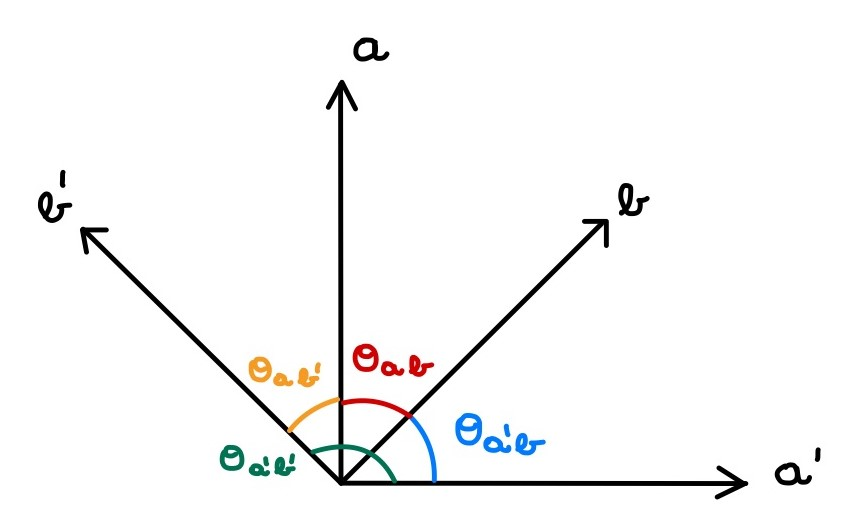
\includegraphics[scale=0.45]{images/CHSH}
    \caption{Direzioni spaziali delle 4 osservabili misurate da Alice e Bob. Si noti che l'apparato di uno è ruotato di 45° rispetto a quello dell'altro perciò $\theta_{a'b} = \theta_{ab} = \theta_{ab'} = 45$° e $\theta_{a'b'} = 135$°.}
    \label{fig:CHSH}
\end{figure}
\noindent Altri esperimenti degni di nota sono quelli condotti da Freedman e Clauser nel 1972, la serie di esperimenti condotti da Aspect negli anni 1981 e 1982, da Tittel e il gruppo Geneva nel 1988 e da Weihs sotto condizioni di località "strettamente einsteniane" nel 1998. La serie di esperimenti sulle disuguaglianze di Bell, di crescente sofisticazione, ha ridotto i critici, che mettono in discussione i risultati, a indicare falle in tale esperimenti, alcune delle quali distorcerebbero i risultati sperimentali in favore della meccanica quantistica. Nel 2015 è stato pubblicato il primo esperimento dichiarato totalmente privo di falle (loopholes), che ha confermato i risultati degli esperimenti precedenti.